\chapter{Сэдвийн судалгаа}

Орчин үеийн программ хангамжийн хөгжүүлэлтэд framework ашиглах нь хөгжүүлэлтийн бүтээмж, кодын зохион байгуулалт, өргөтгөх боломж болон засвар үйлчилгээний чанарт чухал нөлөө үзүүлдэг. Framework нь давтагддаг үйлдлүүдийг автоматжуулах, нийтлэг архитектурын шийдлийг бэлэн байдлаар санал болгох, хөгжүүлэгчийн бичих шаардлагатай кодын хэмжээг бууруулах үндсэн зорилготой байдаг.

Ялангуяа backend систем боловсруулах орчинд framework-ийн үүрэг илүү тодорхой харагддаг. Учир нь backend хөгжүүлэлтэд объектын удирдлага, өгөгдлийн боловсруулалт, хүсэлт хариуны зохицуулалт, бүрэлдэхүүн хоорондын хамаарал зэрэг асуудлууд байнга давтагдан гарч ирдэг. Ийм нөхцөлд framework ашигласнаар системийн бүтэц илүү цэгцтэй, дахин ашиглагдах боломжтой, өргөтгөхөд хялбар хэлбэрт ордог.

Java экосистемд хамгийн өргөн хэрэглэгддэг backend framework-үүдийн нэг нь Spring Framework юм. Spring нь Inversion of Control, Dependency Injection, annotation-д суурилсан тохиргоо зэрэг зарчмуудыг ашигласнаар хөгжүүлэгчид системийн үндсэн бизнес логик дээр төвлөрөх боломжийг олгодог. Иймээс Spring Framework-ийн дотоод ажиллагааны суурь ойлголтууд болох IoC, DI, annotation, reflection зэрэг механизмуудыг судлах нь энэхүү дипломын ажлын сэдэвтэй шууд холбоотой юм.

\newpage
\section{Dependency Injection болон Inversion of Control зарчмын судалгаа}

\subsection{Inversion of Control зарчим}

Inversion of Control (IoC) нь объектуудын үүсэлт, удирдлага,
хамаарлын шийдлийг программын үндсэн логикоос салгаж, тусгай
container эсвэл framework-ээр удирдуулах архитектурын зарчим
юм.
Уламжлалт аргаар объектууд хоорондоо шууд хамааралтайгаар
үүсгэгддэг бол IoC зарчмын үед тухайн удирдлага гаднаас
хийгддэг.

IoC зарчмыг ашигласнаар бүрэлдэхүүн хоорондын хамаарал сул
болж, кодын уян хатан байдал сайжирдаг. Мөн том хэмжээний
системд объектуудын удирдлага төвлөрсөн байдлаар зохион
байгуулагддаг тул өргөтгөл, засвар үйлчилгээ хийхэд хялбар
болдог.\footnote{Spring Framework Documentation.
\textit{Introduction to the Spring IoC Container and Beans}.
\url{https://docs.spring.io/spring-framework/reference/core/beans/introduction.html}}

\begin{figure}[H]
    \centering
    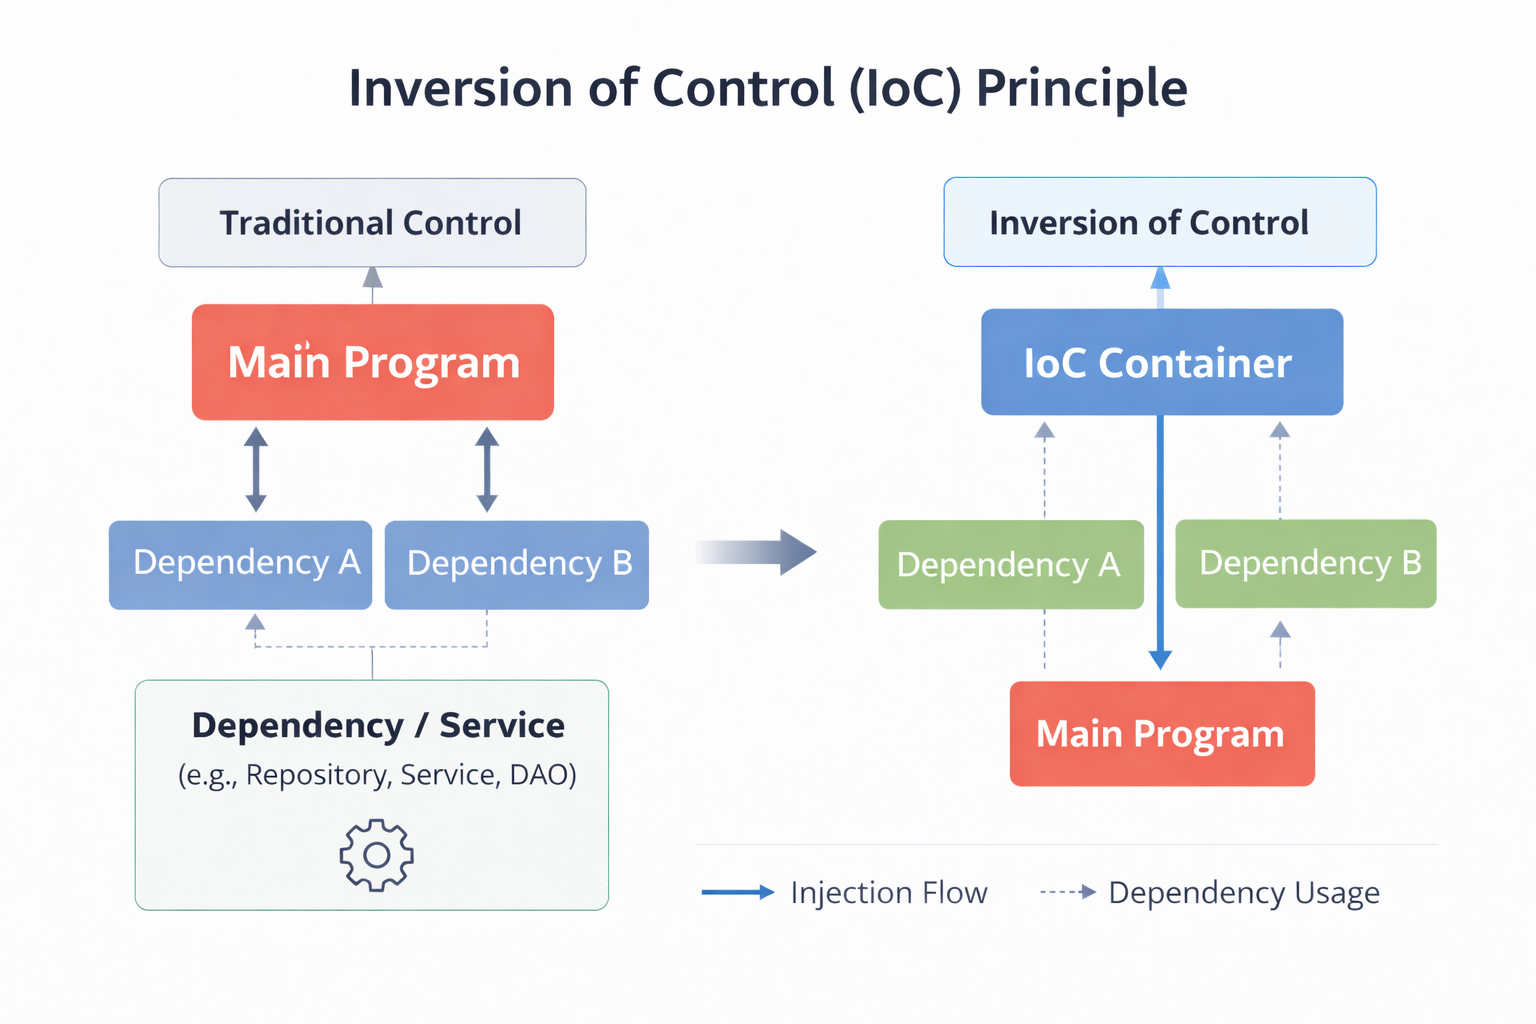
\includegraphics[width=0.8\textwidth]{images/IoC_principle.png}
    \caption{IoC(Inversion of Control) зарчим}
    \label{fig:IoC_principle}
\end{figure}
Дээрх~\ref{fig:IoC_principle}-р зурагт уламжлалт
удирдлага болон IoC зарчмын үндсэн ялгааг харуулав.
Уламжлалт аргаар \texttt{Main Program} нь
\texttt{Dependency A} болон \texttt{Dependency B}-г
өөрөө үүсгэж, шууд удирддаг. Харин IoC зарчмын үед
\texttt{IoC Container} нь dependency-уудыг удирдаж,
\texttt{Main Program}-д шаардлагатай хамаарлыг
гаднаас оруулдаг.

\subsection{Dependency Injection зарчим}

\textbf{Dependency Injection (DI)} нь нэг объектод шаардлагатай өөр объект буюу хамаарлыг тухайн объект өөрөө үүсгэхийн оронд гаднаас оруулах аргачлал юм.Энэ нь \textbf{(IoC)}  хяналтын удирдлагыг зарчим дээр суурилсан \textbf{(design pattern)} үлгэр загвар юм. \footnote{Gamma, E.,
Helm, R., Johnson, R., \& Vlissides, J. (1994).
\textit{Design Patterns: Elements of Reusable Object-Oriented
Software}. Addison-Wesley.}


DI ашигласнаар:
\begin{itemize}
    \item классуудын хоорондын хамаарал сулрах,
    \item тестлэх ажиллагаа хялбарших,
    \item кодын дахин ашиглалт нэмэгдэх,
    \item системийн өргөтгөх боломж сайжрах
\end{itemize}
давуу талууд бий болдог.

\begin{figure}[H]
    \centering
    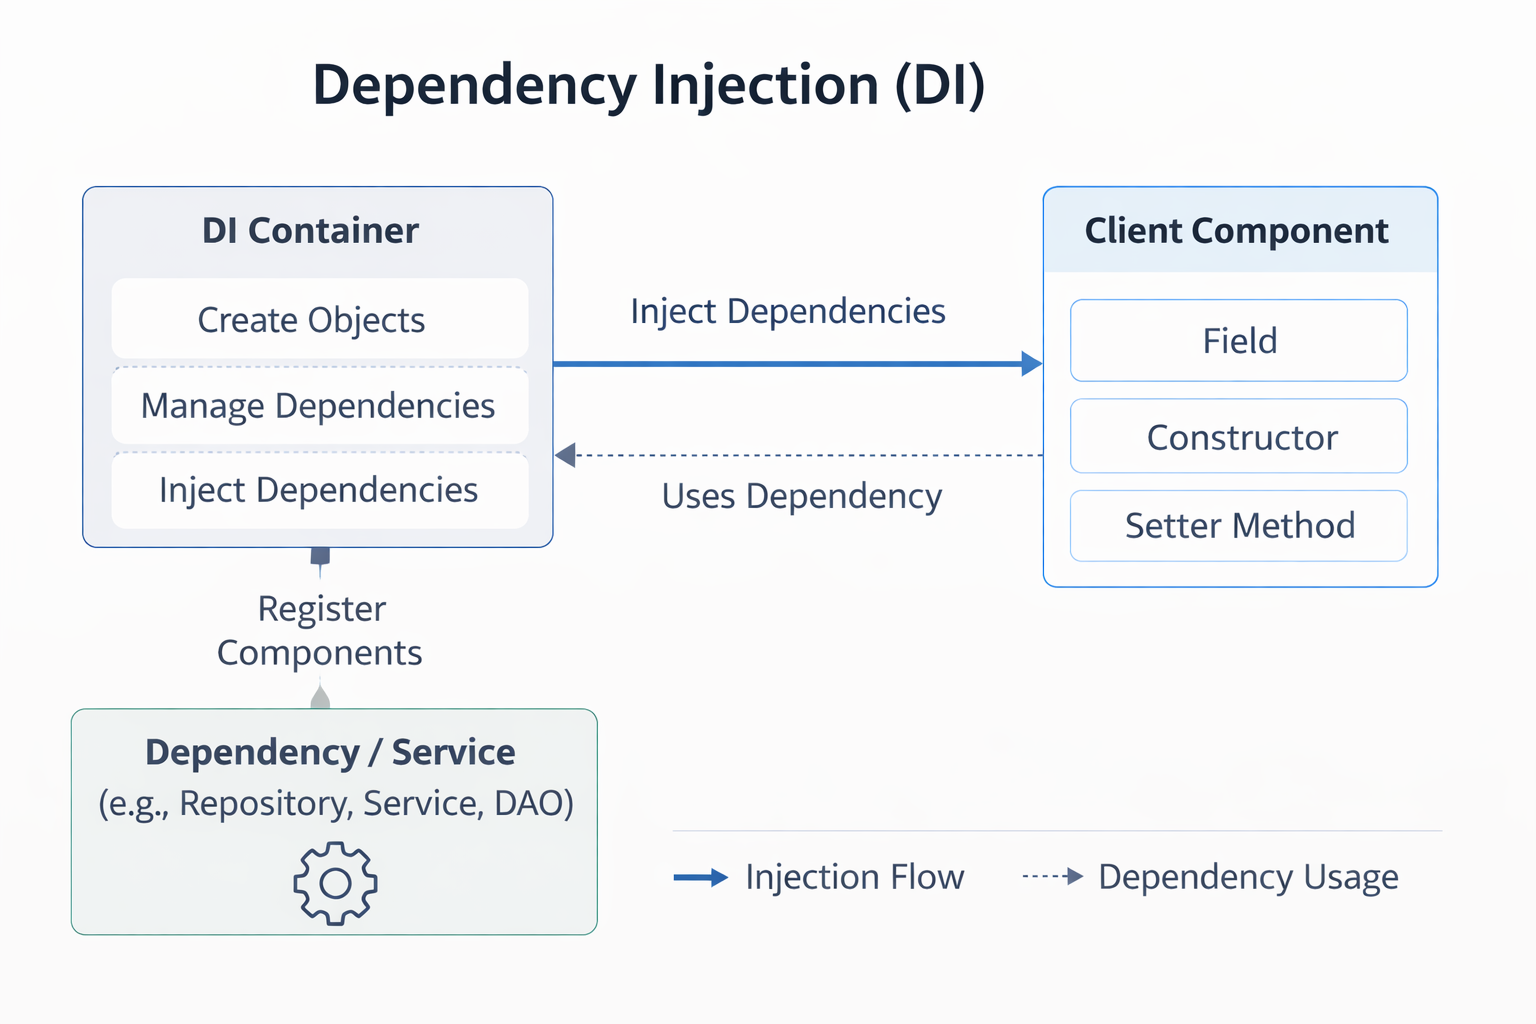
\includegraphics[width=0.8\textwidth]{images/di_principle1.png}
    \caption{DI(Dependency Injection) зарчим}
    \label{fig:di_principle1}
\end{figure}
~\ref{fig:di_principle1}-р зурагт Dependency Injection-ийн
үндсэн механизмыг харуулав. \texttt{DI Container} нь
объект үүсгэх, dependency удирдах, inject хийх гэсэн
гурван үндсэн үүрэг гүйцэтгэнэ. \texttt{Dependency /
Service} буюу \texttt{Repository}, \texttt{Service},
\texttt{DAO} зэрэг бүрэлдэхүүнүүдийг container-д
бүртгэсний дараа \texttt{Client Component}-д шаардлагатай
dependency-г field, constructor эсвэл setter method
хэлбэрээр inject хийдэг.
\newpage


\subsection{Dependency Injection хэрэгжүүлэх үндсэн аргууд}

Dependency Injection нь объект хоорондын хамаарлыг тухайн объект өөрөө үүсгэхийн оронд гаднаас нь нийлүүлэх аргачлал юм. Java болон Spring орчинд dependency injection-ийг хэрэгжүүлэх хамгийн түгээмэл 3 арга байдаг. Үүнд constructor injection, setter injection, field injection орно.

\subsubsection{Constructor Injection}

Constructor Injection нь объект үүсэх мөчид шаардлагатай бүх хамаарлыг байгуулагч функцээр дамжуулан олгодог арга юм. Энэ арга нь dependency-үүдийг заавал дамжуулах шаардлагатай нөхцөлд хамгийн тохиромжтой бөгөөд immutable бүтэц үүсгэх боломжтой.

\begin{lstlisting}[language=Java, caption={Constructor Injection жишээ}, label={lst:constructor-injection}]
interface UserRepository {
    String findUserById(int id);
}

class UserRepositoryImpl implements UserRepository {
    @Override
    public String findUserById(int id) {
        return "User: " + id;
    }
}

class UserService {
    private final UserRepository userRepository;

    public UserService(UserRepository userRepository) {
        this.userRepository = userRepository;
    }

    public void printUser(int id) {
        System.out.println(userRepository.findUserById(id));
    }
}

public class Main {
    public static void main(String[] args) {
        UserRepository repo = new UserRepositoryImpl();
        UserService service = new UserService(repo);
        service.printUser(1);
    }
}
\end{lstlisting}

Энэ аргын үед \texttt{UserService} класс нь \texttt{UserRepository} хамаарлаа байгуулагч функцээрээ дамжуулан авч байна. Иймээс тухайн объект dependency-гүйгээр үүсэх боломжгүй болж, илүү найдвартай бүтэц бүрддэг.


\newpage
\subsubsection{Setter Injection}

Setter Injection нь объектыг эхлээд үүсгээд, дараа нь setter гишүүн функцыг ашиглан dependency-г оноодог арга юм. Энэ нь optional dependency буюу хамаарал заавал хэрэгтэй бус үед хэрэглэхэд тохиромжтой.

\begin{lstlisting}[language=Java, caption={Setter Injection жишээ}, label={lst:setter-injection}]
interface PaymentService {
    void pay(double amount);
}

class CreditCardPaymentService implements PaymentService {
    @Override
    public void pay(double amount) {
        System.out.println("Paid with credit card: " + amount);
    }
}

class OrderService {
    private PaymentService paymentService;

    public void setPaymentService(PaymentService paymentService) {
        this.paymentService = paymentService;
    }

    public void checkout(double amount) {
        paymentService.pay(amount);
    }
}

public class Main {
    public static void main(String[] args) {
        PaymentService payment = new CreditCardPaymentService();

        OrderService orderService = new OrderService();
        orderService.setPaymentService(payment);

        orderService.checkout(150.0);
    }
}
\end{lstlisting}

Энэ жишээнд \texttt{OrderService} объект эхлээд үүсэж, дараа нь \texttt{setPaymentService()} method-оор dependency-г авч байна. Иймээс dependency-г runtime үед өөрчлөх, солих боломжтой байдаг.


\newpage
\subsubsection{Field Injection}

Field Injection нь dependency-г класс доторх талбарт шууд оноох арга юм. Framework-үүд, ялангуяа Spring нь annotation ашиглан энэ аргыг хэрэгжүүлдэг. Кодын хувьд богино, ойлгомжтой боловч тестлэх болон dependency-г ил тод харахад сул талтай.

\begin{lstlisting}[language=Java, caption={Field Injection жишээ}, label={lst:field-injection}]
import org.springframework.beans.factory.annotation.Autowired;
import org.springframework.stereotype.Component;
import org.springframework.stereotype.Service;

interface NotificationService {
    void send(String message);
}

@Component
class EmailNotificationService implements NotificationService {
    @Override
    public void send(String message) {
        System.out.println("Email sent: " + message);
    }
}

@Service
class AlertService {

    @Autowired
    private NotificationService notificationService;

    public void alertUser() {
        notificationService.send("System alert!");
    }
}
\end{lstlisting}

Энэ жишээнд \codeword{AlertService} класс доторх
\codeword{notificationService} талбарт \codeword{@Autowired}
annotation ашиглан dependency injection хийж байна. Хөгжүүлэгч тухайн
dependency-г гараар \codeword{new} ашиглан үүсгэхгүй, харин framework
автоматаар оноож өгдөг.

\subsection{Аргуудын харьцуулалт}

Dependency Injection-ийн дээрх 3 аргыг дараах байдлаар харьцуулан авч үзэж болно.

\begin{table}[H]
\centering
\small
\renewcommand{\arraystretch}{1.2}
\caption{Dependency Injection аргуудын харьцуулалт}
\label{tab:di-comparison}
\begin{tabularx}{\textwidth}{|L{0.22\textwidth}|Y|Y|}
\hline
\textbf{Арга} & \textbf{Давуу тал} & \textbf{Сул тал} \\
\hline
Constructor Injection & Dependency заавал олгогдоно, test хийхэд хялбар, immutable бүтэц үүсгэнэ & Dependency олон бол constructor урт болно \\
\hline
Setter Injection & Optional dependency-д тохиромжтой, runtime үед солих боломжтой & Dependency дутуу үлдэх эрсдэлтэй \\
\hline
Field Injection & Код богино, annotation ашиглахад хялбар & Test хийхэд хэцүү, framework-ээс хэт хамааралтай \\
\hline
\end{tabularx}
\normalsize
\renewcommand{\arraystretch}{1}
\end{table}

\newpage
\subsection{Дүгнэлт}

Dependency Injection-ийг хэрэгжүүлэх 3 үндсэн арга байдгаас constructor injection нь хамгийн найдвартай, тестлэхэд хялбар арга гэж үзэгддэг. Setter injection нь optional dependency-д тохиромжтой бол field injection нь annotation-д суурилсан framework-үүдэд өргөн хэрэглэгддэг. Энэхүү судалгааны ажлын хүрээнд annotation болон reflection механизмд тулгуурласан dependency injection framework хэрэгжүүлэх тул field injection арга нь онцгой ач холбогдолтой юм.
\newpage
\section{Annotation болон Reflection механизмын судалгаа}

\subfile{ann_refl}
\newpage




\section{Ижил төрлийн framework-үүдийн судалгаа}

Dependency Injection механизмыг хэрэгжүүлсэн түгээмэл framework-үүдэд Spring Framework, Google Guice, Jakarta CDI зэрэг орно. Эдгээр framework-үүд нь объектын хамаарлыг удирдах, container ашиглан объект үүсгэх, configuration боловсруулах зэрэг нийтлэг үүрэгтэй боловч хэрэгжүүлэлтийн арга барил, цар хүрээ, өргөтгөх боломжийн хувьд ялгаатай.

\subsection{Spring Framework}

Spring Framework нь Java экосистем дэх хамгийн өргөн хэрэглэгддэг framework-үүдийн нэг бөгөөд dependency injection, aspect-oriented programming, transaction management, web development зэрэг олон боломжийг агуулдгаараа онцлогтой. Энэ framework нь annotation-д суурилсан тохиргоо болон IoC container ашиглан объектуудын удирдлагыг төвлөрсөн байдлаар зохион байгуулдаг.

\begin{figure}[H]
    \centering
    
\includegraphics[width=0.22\textwidth]{images/spring_frame.png}
    \caption{Spring Framework}
    \label{fig:spring-framework}
\end{figure}

\newpage
\subsection{Google Guice}

Google Guice нь dependency injection-д чиглэсэн, харьцангуй энгийн бүтэцтэй Java framework юм. Энэ нь Spring-тэй харьцуулахад боломжийн хүрээ бага боловч DI зарчмыг ойлгох, жижиг болон дунд хэмжээний системд хэрэгжүүлэхэд тохиромжтой.\footnote{Google. (2024).
\textit{Google Guice: A lightweight dependency injection
framework for Java}. GitHub.
\url{https://github.com/google/guice/wiki/Motivation}}

\begin{figure}[H]
    \centering
    
\includegraphics[width=0.4\textwidth]{images/google_guice.png}
    \caption{Google Guice}
    \label{fig:google-guice}
\end{figure}

\subsection{Jakarta CDI}

Jakarta CDI (Contexts and Dependency Injection) нь enterprise Java орчинд dependency injection болон component lifecycle management хэрэгжүүлэх стандарт тодорхойлолт юм. Энэ нь Java enterprise орчны албан ёсны стандартуудын нэг хэсэг бөгөөд enterprise түвшний системд өргөн ашиглагддаг.

\begin{figure}[H]
    \centering
    
\includegraphics[width=0.4\textwidth]{images/jakarta.png}
    \caption{Jakarta CDI}
    \label{fig:jakarta-cdi}
\end{figure}
\subsection{Framework-үүдийн харьцуулалт}

\begin{table}[H]
\centering
\caption{Түгээмэл DI framework-үүдийн харьцуулалт}
\label{tab:framework-comparison}
\begin{tabular}{|p{3.5cm}|p{4cm}|p{5cm}|}
\hline
\textbf{Framework} & \textbf{Үндсэн зориулалт} & \textbf{Онцлог} \\
\hline
Spring Framework & Иж бүрэн application framework & IoC, DI, annotation, web, data access зэрэг өргөн боломжтой \\
\hline
Google Guice & DI чиглэлийн framework & Энгийн бүтэцтэй, dependency injection-д төвлөрсөн \\
\hline
Jakarta CDI & Java enterprise стандарт DI & Enterprise орчинд component lifecycle болон injection дэмждэг \\
\hline
\end{tabular}
\end{table}

Хүснэгт~\ref{tab:framework-comparison}-оос харахад Spring Framework нь хамгийн өргөн боломжтой, харин Google Guice нь илүү төвлөрсөн DI шийдэл болох нь ажиглагдана.

\newpage
\section{Ашиглагдах программчлалын хэлний судалгаа}

Энэхүү дипломын ажлын хэрэгжүүлэлтэд Java программчлалын хэлийг ашигласан. Java хэл нь объект хандалтат загварчлалыг бүрэн дэмждэг, өргөн хөгжүүлэлтийн экосистемтэй, annotation болон reflection механизмыг хэлний түвшинд агуулдаг тул судалгааны сэдэвтэй шууд нийцэж байна.

Java хэлний үндсэн давуу талд:
\begin{itemize}
    \item объект хандалтат бүтэц,
    \item annotation болон reflection дэмжлэг,
    \item олон платформ дээр ажиллах чадвар,
    \item framework хөгжүүлэхэд тохиромжтой сангууд,
    \item өргөн хэрэглээ, баримтжуулалт
\end{itemize}
зэрэг орно.

\begin{figure}[H]
    \centering
    
\includegraphics[width=0.22\textwidth]{images/java-logo.png}
    \caption{Java программчлалын хэл}
    \label{fig:java-language}
\end{figure}

\newpage
\section{Ашиглагдах технологи, хэрэгслүүдийн судалгаа}

% \subsection{Spring Framework}

% Spring Framework нь энэхүү ажлын хэрэгжүүлэлтийн шууд хэрэгсэл биш боловч судалгааны жишиг framework байдлаар ашиглагдана. Өөрөөр хэлбэл, хэрэгжүүлэх DI Framework-ийн архитектур, dependency injection механизм, annotation боловсруулах логикийг ойлгоход Spring Framework гол жишиг суурь болно.

\subsection{Maven}

Maven нь Java төслийн dependency management болон build management хийх хэрэгсэл юм. Энэхүү ажлын хүрээнд төслийн сангуудыг удирдах, бүтэц зохион байгуулалтыг стандартчилах, хэрэгжүүлэлтийг эмх цэгцтэй байлгах зорилгоор ашиглана.\footnote{Apache Software Foundation.
(2024). \textit{Maven -- Welcome to Apache Maven}.
\url{https://maven.apache.org/index.html}}

\begin{figure}[H]
    \centering
    
\includegraphics[width=0.22\textwidth]{images/maven.png}
    \caption{Maven builder}
    \label{fig:maven-logo}
\end{figure}

\subsection{JUnit}

JUnit нь Java орчинд unit test бичих түгээмэл хэрэгсэл юм. Хэрэгжүүлсэн framework-ийн үндсэн функцүүд болох annotation илрүүлэлт, объект үүсгэх, dependency injection хийх ажиллагааг шалгахын тулд JUnit ашиглах боломжтой.

\begin{figure}[H]
    \centering
    
\includegraphics[width=0.4\textwidth]{images/JUnit.png}
    \caption{JUnit test}
    \label{fig:junit-logo}
\end{figure}
\subsection{Хөгжүүлэлтийн орчин}

Хөгжүүлэлтийн орчноор IntelliJ IDEA эсвэл Eclipse зэрэг Java хөгжүүлэлтийг дэмждэг integrated development environment ашиглаж болно. Эдгээр орчин нь код бичих, dependency удирдах, debug хийх, тест ажиллуулах зэрэг олон талын боломж олгодог.\footnote{JetBrains. (2024).
\textit{IntelliJ IDEA: The Leading Java and Kotlin IDE}.
\url{https://www.jetbrains.com/idea/}}

\begin{figure}[H]
    \centering
    \begin{minipage}{0.45\textwidth}
        \centering
        
\includegraphics[width=0.8\textwidth]{images/intellij.png}
        \caption{IntelliJ IDEA}
        \label{fig:intellij}
    \end{minipage}
    \hfill
    \begin{minipage}{0.45\textwidth}
        \centering
        
\includegraphics[width=0.8\textwidth]{images/eclipse.png}
        \caption{Eclipse}
        \label{fig:eclipse}
    \end{minipage}
\end{figure}

\subsection{Git болон GitHub}

Git нь хувилбар удирдлагын систем бөгөөд төслийн хөгжүүлэлтийн явц дахь өөрчлөлтүүдийг хянахад ашиглагдана. GitHub нь тухайн repository-г хадгалах, хувилбаруудыг удирдах, хөгжүүлэлтийн явцыг баримтжуулахад дэмжлэг үзүүлнэ.

\begin{figure}[H]
    \centering
    
\includegraphics[width=0.4\textwidth]{images/git.png}
    \caption{Git GitHub}
    \label{fig:git-github}
\end{figure}

\newpage
\section{Системийн ерөнхий шийдлийн судалгаа}

Энэхүү дипломын ажлын хүрээнд хэрэгжүүлэх framework нь annotation болон reflection механизмд тулгуурласан суурь түвшний dependency injection framework юм. Иймээс шийдлийн судалгааны хэсэгт ижил зарчмаар ажилладаг Spring Framework-ийн IoC container, bean удирдлага, configuration, dependency injection болон bean scope-ийн ойлголтуудыг авч үзэх нь зүйтэй. Spring нь enterprise түвшний иж бүрэн framework боловч түүний үндсэн IoC/DI зарчим нь энэхүү ажлын хэрэгжүүлэлтийн логиктой шууд холбоотой.

\subsection{Spring Framework-ийн IoC container}

Spring framework-ийн IoC container нь объектыг үүсгэх, тохируулах, dependency-г шийдэх үндсэн үүргийг гүйцэтгэдэг. Энэ container-ийн суурь ойлголтууд хэрэгжүүлэлтүүд нь \texttt{BeanFactory} болон \texttt{ApplicationContext} юм.\footnote{Spring Framework Documentation.
(2024). \textit{The IoC Container}.
\url{https://docs.spring.io/spring-framework/reference/
core/beans.html}}

\subsubsection{BeanFactory}

\texttt{BeanFactory} нь IoC container-ийн хамгийн суурь түвшний root interface бөгөөд bean объектыг үүсгэх, хадгалах, буцаах үндсэн үүрэгтэй. Үүний онцлог нь bean-ийг ихэвчлэн \texttt{getBean()} дуудагдсан үед үүсгэдэгт оршино. Иймээс санах ойн хэрэглээг хэмнэх боломжтой боловч орчин үеийн Spring төслүүдэд дангаар нь түгээмэл ашигладаггүй.

\begin{lstlisting}[language=Java, style=mystyle, caption={BeanFactory ашигласан жишээ}, label={lst:beanfactory-example}]
BeanFactory factory =
    new XmlBeanFactory(new ClassPathResource("beans.xml"));

UserService service = factory.getBean(UserService.class);
\end{lstlisting}

\subsubsection{ApplicationContext}

\texttt{ApplicationContext} нь \texttt{BeanFactory}-ийг өргөтгөсөн интерфейс бөгөөд bean удирдлагаас гадна event system, resource management, annotation support зэрэг нэмэлт боломжуудыг олгодог. Орчин үеийн Spring төслүүдэд ихэвчлэн \texttt{ApplicationContext} ашиглагддаг.

\begin{lstlisting}[language=Java, caption={ApplicationContext ашигласан жишээ}, label={lst:applicationcontext-example}]
ApplicationContext context =
    new ClassPathXmlApplicationContext("applicationContext.xml");

UserService service = context.getBean(UserService.class);
\end{lstlisting}

Иймээс энэхүү дипломын ажлын хүрээнд хэрэгжүүлэх DI framework-ийн container ойлголтыг тодорхойлохдоо \texttt{ApplicationContext}-ийн ажиллагааг жишиг болгон авч үзэх боломжтой.

\subsection{Bean болон container-д бүртгэгдэх классууд}

IoC container-аар удирдагдаж буй объектыг \textit{bean} гэж нэрлэдэг. Spring-д зөвхөн тодорхой annotation-оор тэмдэглэгдсэн класс эсвэл \texttt{@Bean} annotation-оор буцаасан объект bean болж бүртгэгдэнэ.

Bean болдог түгээмэл annotation-ууд:
\begin{itemize}
    \item \texttt{@Component}
    \item \texttt{@Service}
    \item \texttt{@Repository}
    \item \texttt{@Controller}
    \item \texttt{@Bean}
\end{itemize}

Жишээ нь:

\begin{lstlisting}[language=Java, caption={Component болон Service annotation ашигласан жишээ}, label={lst:component-service-example}]
@Component
public class UserRepositoryImpl implements UserRepository {
    public String findUser(int id) {
        return "Хэрэглэгч: " + id;
    }
}

@Service
public class UserService {
    private final UserRepository repo;

    @Autowired
    public UserService(UserRepository repo) {
        this.repo = repo;
    }
}
\end{lstlisting}

Харин дараах annotation-ууд нь bean бүртгэхгүй:

\begin{itemize}
    \item \texttt{@Override}
    \item \texttt{@Deprecated}
    \item \texttt{@SuppressWarnings}
    \item \texttt{@Autowired}
    \item \texttt{@Getter}, \texttt{@Setter}
\end{itemize}

Өөрөөр хэлбэл зарим annotation нь зөвхөн metadata өгдөг бол зарим нь container-ийн бодит ажиллагаанд оролцдог.

\subsection{Spring configuration хийх үндсэн аргууд}

Spring framework-д container-д ямар объект бүртгэх, dependency-г хэрхэн шийдэхийг configuration-оор тодорхойлдог. Үүнийг хэрэгжүүлэх хэд хэдэн үндсэн арга бий.

\subsubsection{XML суурилсан configuration}

Spring-ийн анхны арга нь bean бүрийг XML файлд тодорхойлох байсан.

\begin{lstlisting}[language=XML, basicstyle=\ttfamily\small, numbers=left, numberstyle=\tiny\color{gray}, frame=single, caption={XML суурилсан bean тодорхойлолтын жишээ}, label={lst:xml-bean-config-example}]
<beans xmlns="http://www.springframework.org/schema/beans">

    <bean id="userRepository"
          class="com.myapp.UserRepositoryImpl"/>

    <bean id="userService"
          class="com.myapp.UserService">
        <constructor-arg ref="userRepository"/>
    </bean>

</beans>
\end{lstlisting}

\begin{lstlisting}[language=XML, basicstyle=\ttfamily\small, numbers=left, numberstyle=\tiny\color{gray}, frame=single, caption={XML configuration ачаалах жишээ}, label={lst:xml-context-loading-example}]
ApplicationContext context =
    new ClassPathXmlApplicationContext("applicationContext.xml");

UserService service = context.getBean(UserService.class);
\end{lstlisting}

Энэ арга нь ойлгомжтой боловч тохиргоо ихсэх тусам XML файл төвөгтэй болдог.

\subsubsection{Annotation-д суурилсан configuration}

Энэ аргад bean болон dependency-г класс дээр annotation ашиглан тодорхойлно.

\begin{lstlisting}[language=Java, frame=single, caption={Annotation-д суурилсан bean бүртгэлтийн жишээ}, label={lst:annotation-config-example}]
@Component
public class UserRepositoryImpl implements UserRepository {
}

@Service
public class UserService {
    private final UserRepository repo;

    @Autowired
    public UserService(UserRepository repo) {
        this.repo = repo;
    }
}
\end{lstlisting}

\begin{lstlisting}[language=XML, basicstyle=\ttfamily\small, numbers=left, numberstyle=\tiny\color{gray}, frame=single, caption={Component scan тохиргооны жишээ}, label={lst:component-scan-example}]
<beans>
    <context:component-scan base-package="com.myapp"/>
</beans>
\end{lstlisting}

Энэ нь XML-ийг багасгаж, код болон тохиргоог ойртуулсан давуу талтай.

\newpage
\subsubsection{Java-д суурилсан configuration}

Орчин үед хамгийн түгээмэл хэрэглэгддэг арга нь Java configuration юм.

\begin{lstlisting}[language=Java, frame=single, caption={Java-д суурилсан configuration жишээ}, label={lst:java-config-example}]
@Configuration
@ComponentScan("com.myapp")
public class AppConfig {

    @Bean
    public UserRepository userRepository() {
        return new UserRepositoryImpl();
    }

    @Bean
    public UserService userService() {
        return new UserService(userRepository());
    }
}
\end{lstlisting}

\begin{lstlisting}[language=Java, frame=single, caption={Java configuration-оос container үүсгэх жишээ}, label={lst:java-context-example}]
ApplicationContext context =
    new AnnotationConfigApplicationContext(AppConfig.class);

UserService service = context.getBean(UserService.class);
\end{lstlisting}

Энэ арга нь XML-ийг бараг бүрэн орлуулсан бөгөөд кодоор configuration удирдах боломж олгодог.

\subsubsection{Spring Boot configuration}

Spring Boot нь дээрх тохиргоонуудыг илүү автоматжуулсан хэлбэрээр хэрэгжүүлдэг.

\begin{lstlisting}[language=Java, frame=single, caption={Spring Boot configuration жишээ}, label={lst:springboot-config-example}]
@SpringBootApplication
public class Main {
    public static void main(String[] args) {
        SpringApplication.run(Main.class, args);
    }
}
\end{lstlisting}

\texttt{@SpringBootApplication} нь \texttt{@Configuration}, \texttt{@ComponentScan} гэсэн ойлголтуудыг нэгтгэн агуулдаг.\footnote{Spring Framework
Documentation. (2024).
\textit{Java-based Container Configuration}.
\url{https://docs.spring.io/spring-framework/reference/
core/beans/java.html}}

\subsection{Dependency Injection ба annotation ашиглалт}

Dependency Injection нь объект өөрийн dependency-г шууд үүсгэхийн оронд container-аас авч ашиглах зарчим юм. Spring-д үүнийг annotation-оор хялбар илэрхийлдэг.

\begin{lstlisting}[language=Java, frame=single, caption={Autowired ашигласан dependency injection жишээ}, label={lst:autowired-example}]
@Service
public class UserService {

    private final UserRepository repo;

    @Autowired
    public UserService(UserRepository repo) {
        this.repo = repo;
    }
}
\end{lstlisting}

Энд \texttt{@Autowired} annotation нь \texttt{UserRepository} төрлийн bean-ийг автоматаар оноож өгнө. Энэ зарчим нь классуудын хамаарлыг сулруулж, турших болон өргөтгөхөд хялбар болгодог.

\subsection{Bean scope}

Bean scope нь тухайн bean хэдэн хувь үүсэх, ямар хугацаанд оршин байхыг тодорхойлдог. Spring-д хэд хэдэн төрөл байдаг боловч энэхүү ажлын хүрээнд дараах хоёр scope хамгийн чухал гэж үзэж болно.

\subsubsection{Singleton scope}

\texttt{Singleton} нь bean зөвхөн нэг удаа үүсэж, container-ийн хүрээнд дахин дахин ижил объектыг буцаана.

\begin{lstlisting}[language=Java,frame=single, caption={Singleton scope ашигласан жишээ}, label={lst:singleton-scope-example}]
@Component
@Scope("singleton")
public class AppConfigManager {
}
\end{lstlisting}

Энэ нь төлөв хадгалдаггүй service төрлийн классуудад тохиромжтой.

\subsubsection{Prototype scope}

\texttt{Prototype} нь bean дуудагдах бүрд шинэ объект үүсгэнэ.

\begin{lstlisting}[language=Java, frame=single, caption={Prototype scope ашигласан жишээ}, label={lst:prototype-scope-example}]
@Component
@Scope("prototype")
public class TempDataHolder {
}
\end{lstlisting}

Энэ нь объект бүр өөрийн төлөвтэй байх шаардлагатай үед илүү тохиромжтой.

\subsection{Хэрэгжүүлэх framework-ийн ерөнхий шийдэлтэй уялдах нь}

Дээрх судалгаанаас үзэхэд Spring Framework-ийн IoC container нь annotation-оор классуудыг илрүүлэх, bean болгон бүртгэх, dependency-г автоматаар шийдэх, объектын амьдралын мөчлөгийг удирдах нэгдсэн механизмыг хэрэгжүүлдэг. Энэхүү дипломын ажлын хүрээнд хэрэгжүүлэх framework нь Spring-ийн бүх боломжийг бүрэн хуулбарлахгүй боловч түүний үндсэн IoC/DI зарчмыг хялбаршуулсан түвшинд хэрэгжүүлэхэд чиглэнэ.

Тодруулбал хэрэгжүүлэх framework-ийн ажиллагааг дараах үе шатуудад авч үзэж болно:
\begin{enumerate}
    \item package эсвэл тодорхой классуудыг scan хийх,
    \item annotation-уудыг илрүүлэх,
    \item component классуудыг container-д бүртгэх,
    \item reflection ашиглан объект үүсгэх,
    \item dependency-г автоматаар оноох,
    \item хэрэглээний түвшинд бэлэн объектыг ашиглах
\end{enumerate}

Иймээс Spring Framework-ийн дээрх шийдлийн судалгаа нь энэхүү ажлын онолын суурь болохын зэрэгцээ хэрэгжүүлэх dependency injection framework-ийн бүтэц, үндсэн боломжуудыг тодорхойлох жишиг загвар болж байна.

\subsection{Dependency graph болон observability-ийн хэрэгцээ}

Орчин үеийн dependency injection framework-үүдийн нэг чухал давуу тал нь зөвхөн dependency-г автоматаар шийдэхэд бус, мөн тухайн dependency бүтэц хэрхэн бүрдэж буйг хөгжүүлэгчид ойлгомжтой байдлаар харах боломж олгодогт оршдог. Ялангуяа backend системийн бүрэлдэхүүн олон болох тусам ямар service ямар repository-г ашиглаж байгаа, аль bean root node болж байгаа, ижил төрлийн bean-үүдийн аль нь inject хийгдэж буй, циклийн эрсдэл хаана байгааг зөвхөн код уншаад ойлгох нь хүндрэлтэй болдог. Ийм нөхцөлд dependency graph буюу dependency tree хэлбэрээр framework-ийн дотоод бүтцийг дүрслэх чадвар нь observability-ийн чухал хэсэг болно.

Spring зэрэг иж бүрэн framework-үүд өөрсдийн startup лог, actuator, bean report зэрэг олон хэрэгслээр дотоод төлөвөө тайлбарлах боломжтой байдаг. Харин энэхүү дипломын ажлын хүрээнд хөгжүүлж буй цэвэр Java SE орчинд ажиллах framework нь гуравдагч талын сан ашиглахгүй байх шаардлагатай тул dependency structure-ийг тайлбарлах тусгай exporter болон visualization логикийг өөрийн түвшинд боловсруулах шаардлага үүснэ. Энэ нь A3 ажлын онолын үндэслэл болж байгаа бөгөөд dependency injection-ийн үр дүнг мод бүтэц, JSON representation, интерактив HTML dashboard-аар харагдуулах нь framework-ийн ойлгомжтой байдал, оношлогоо, туршилтын баталгаажуулалтын чанарыг мэдэгдэхүйц өсгөнө.

Иймээс энэхүү судалгааны ажлын хувьд dependency injection механизмыг ``шийддэг'' байх нь хангалтгүй, харин түүний үр дүнг ``тайлбарлаж чаддаг'' байх нь дараагийн логик алхам гэж үзэж болно. Энэ үзэл баримтлал нь дараагийн бүлгүүдэд тайлбарлах dependency tree үүсгэлт, DFS цикл илрүүлэлт, JSON болон HTML visualization-ийн хэрэгжүүлэлтийн онолын суурь болж байна.

\begin{figure}[H]
    \centering
    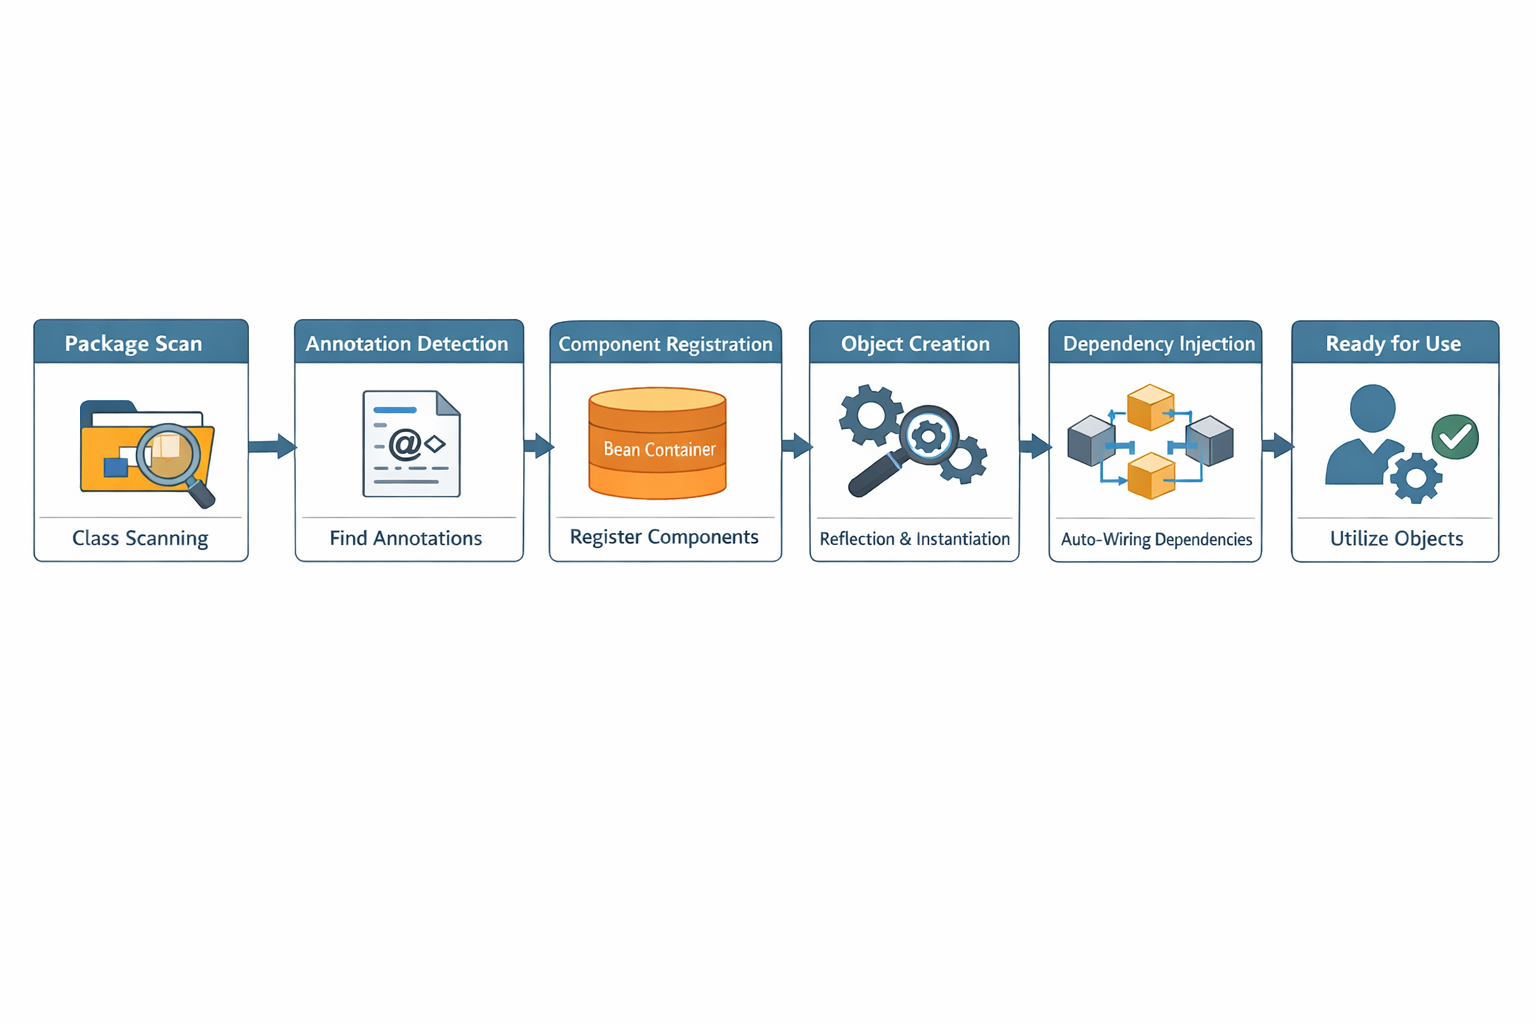
\includegraphics[width=0.85\textwidth]{images/framework-flow}
    \caption{Хэрэгжүүлэх DI Framework-ийн ерөнхий ажиллагааны зураглал}
    \label{fig:framework-architecture}
\end{figure}

Зураг~\ref{fig:framework-architecture}-т хэрэгжүүлэх framework-ийн ерөнхий урсгал, үндсэн бүрэлдэхүүн хэсгүүдийн хамаарлыг харуулсан.

\section{Бүлгийн дүгнэлт}

Энэ бүлэгт энэхүү дипломын ажлын хэрэгжүүлэлтийн онолын болон технологийн суурь нөхцөлүүдийг судлав. Үүнд framework-ийн ерөнхий ойлголт, IoC болон DI зарчим, annotation болон reflection механизм, ижил төрлийн framework-үүдийн онцлог, мөн хэрэгжүүлэлтэд ашиглагдах Java хэл, Maven, JUnit, Git зэрэг технологи, хэрэгслүүдийг авч үзлээ. Судалгааны үр дүнд annotation болон reflection-д суурилсан суурь түвшний DI Framework хэрэгжүүлэхэд Java орчин хамгийн тохиромжтой бөгөөд Spring Framework нь судалгааны жишиг болгон ашиглагдах үндэслэлтэй болох нь тогтоогдож байна.